%%%%%%%%%%%%%%%%%%%%%%%%%%%%%%%%%%%%%%%%%%%%%%%%%%%%%%%%%%%%%%%%
%% IFJ.tex - dokumentace k projektu z predmetu IFJ a IAL 2006 %%
%% Kodovani: ISO_8859-2
%%%%%%%%%%%%%%%%%%%%%%%%%%%%%%%%%%%%%%%%%%%%%%%%%%%%%%%%%%%%%%%%

\documentclass[11pt, notitlepage]{article}

%% import vlastniho stylu a potrebnych baliku
\usepackage{IFJ}

%%% informace o dokumentu %%%

\title{Interpret imperativního jazyka IFJ06}

\varianta{Projekt z předmětů IFJ a IAL 2006 \\
          varianta zadání d/3, tým 6}

\author{
Lukáš Maršík, xmarsi03    (20\%\,bodů) \\
Libor Polčák, xpolca03    (20\%\,bodů) \\
Boris Procházka, xproch63 (20\%\,bodů) \\
Martin Tomec, xtomec05    (20\%\,bodů) \\
Petr Zemek,   xzemek02    (20\%\,bodů) \\
}
\def\@fitname{Fakulta informačních technologií}
\rozsireni{prediktivní syntaktická analýza \\
   víceřádkové komentáře /* */}


%%%%%%%%%%%%%%%%%%%%%%%%%%%%%%%%%%%%%%%%%%%%%%%%%%%%%%%%%%%%%%%%%%%%%%%%%%%%%
\begin{document}

%% titulni strana
\maketitle


%% cislovani stran FIXME
\pagestyle{plain}
\setcounter{page}{2}

%%%%%%%%%%%%%%%%%%%%%%%%%%%%%%%%%%%%%%%%%%%%%%%%%%%%%%%%%%%%%%%%%%%%%%%%%%%%%
% Vlastni text

\section{Úvod}
Tato dokumentace popisuje návrh a implementaci interpretu imperativního jazyka IFJ06. Naše varianta byla d/3, takže tabulka symbolů byla implementována hashovací tabulkou a k řazení byl použit algoritmus Shellsort.

Následuje stručný popis jednotlivých součástí našeho programu a metod použitých při vývoji.

\section{Práce v týmu a komunikace}

Každé úterý jsme se scházeli, abychom mohli prodiskutovat návrh programu a jeho jednotlivých částí, o přestávce na přednáškách jsme pak projednávali implementační detaily a procházeli specifikace v zadání.

Internetová komunikace (ICQ/IRC/Jabber) byla také důležitá, protože jsme pracovali v odlišných lokalitách, nebyla ústní domluva možná. Ke správě zdrojových souborů jsme využívali SVN\footnote{http://subversion.tigris.org/} repositář na serveru merlin, mohli jsme tak souběžně pracovat na zdrojových souborech prakticky bez omezení a urychlovalo to aktualizace a opravy chyb.

Byl také zaveden tzv. \uv{kódovací standard} - specifikace formátování k zachování konzistence pojmenování proměnných, odsazování atd. Během vývoje jsme se navzájem ihned upozorňovali, pokud jsme v programu nalezli chybu a informovali správce daného modulu - při drobnější chybě ji stačilo opravit přímo.


\section{Lexikální analýza}

Při tvorbě lexikálního analyzátoru bylo nejprve nutné převést jenotlivé lexémy (popsané regularními výrazy) na deterministický konečný automat. Dále jsme určili množinu speciálních identifikátorů - množinu klíčových slov. Automat obsahuje rozšíření o možnost blokových komentářů. Celkové schéma automatu popisuje vložený obrázek.

\begin{center}
 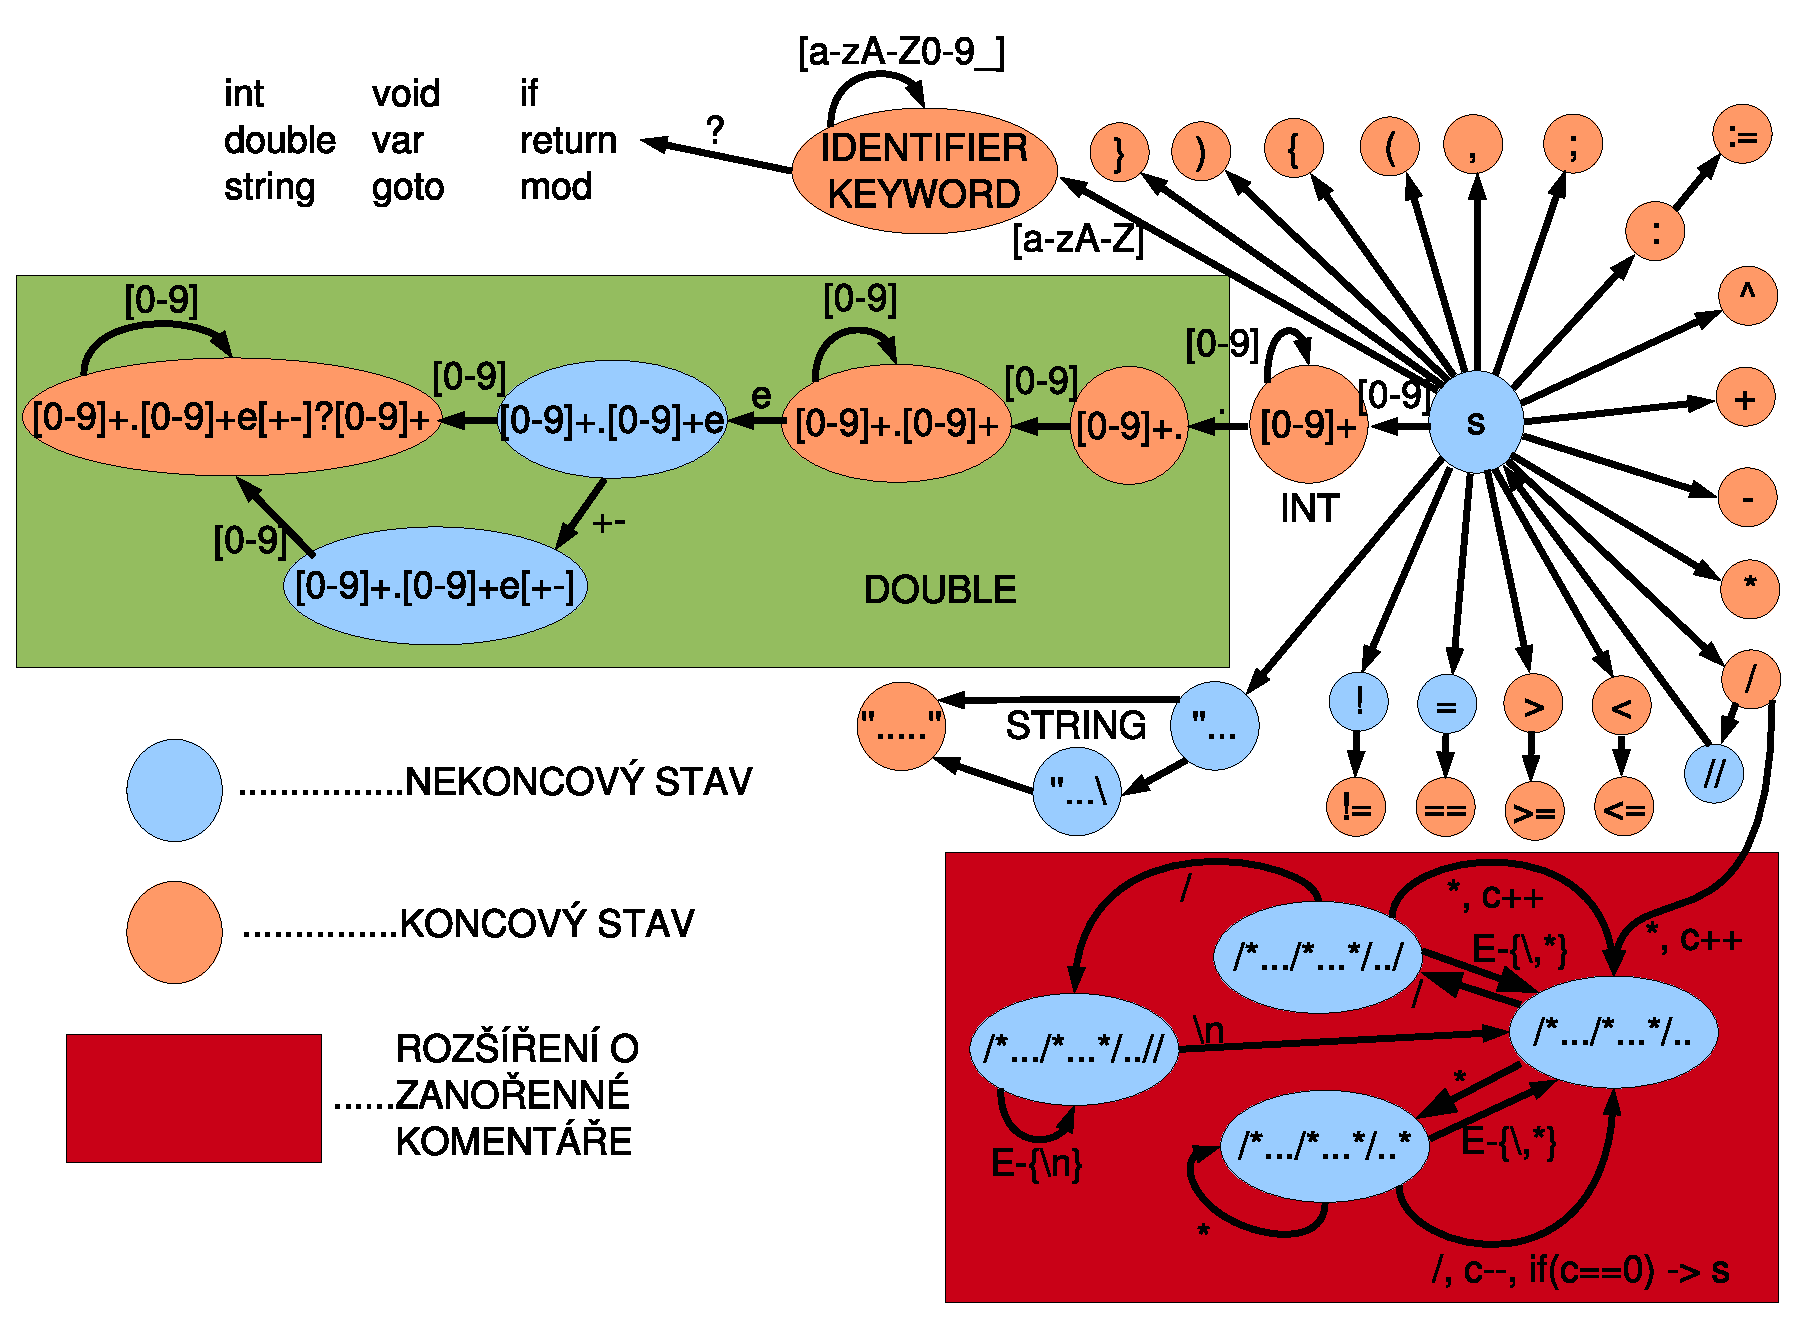
\includegraphics[scale=0.5]{include/scanner.eps}
\end{center}

Automat byl implementován nekonečným cyklem. Pokus o vyskočení z cyklu v nekoncovém stavu znamená chybný lexém a konec programu. Automat je schopen načítat lexémy libovolné délky, kontroluje přetečení při konverzi a zaznamenává pozici v načítaném souboru.


\section {Syntaktická a sémantická analýza}

Syntaktická analýza (dále jen SA) je \uv{srdcem} našeho programu a skládá se ze dvou částí: \textbf{prediktivní SA} (použita pro kontrolu deklarací/definic, těla funkcí a volání funkce)
a \textbf{precedenční SA} (analýza výrazů). Principem je křížové volání těchto dvou částí v průběhu analýzy. Ze sémantických důvodů bylo nutné SA rozdělit na dvě fáze, a to deklarace (funkcí a globálních proměnných) a definice (tělo funkce, její parametry a lokální proměnné).

SA spolupracuje s lexikální analýzou a tabulkou symbolů (dále jen TS). Byla vytvořena speciální funkce, která volá lexikální analyzátor, provádí část sémantické kontroly a spolupracuje s TS (číst zdrojový text je nutné ve více částech SA).

Obě analýzy používají shodné struktury, které jsou implementovány dostatečně obecně. Pravá strana pravidel je implementována jako pole, usnadňuje to převrácení pravidla při vkládání na zásobník v prediktivní SA a kontrolu při redukci v precedenční SA.

\subsection{Prediktivní SA}

Tato metoda je založena na LL tabulce (která navíc obsahuje speciální pravidlo, které značí, že následuje výraz a tudíž budeme volat precedenční SA na jeho zpracování).
Volání funkce řeší právě tato metoda - proto není např. nutné v tělě funkce kontrolovat, zda příkaz začíná voláním funkce (normálně by se musela volat precedenční SA), nebo se jedná o výraz (syntaktická chyba)

Vlastní algoritmus používá zásobník na terminály a non-terminály se standardními operacemi (push, top, pop, ...) - implementován jednosměrně vázaným seznamem.

Je nutné uchovávat některé údaje, např. poslední použité pravidlo, poslední načtený identifikátor, jeho datový typ a index na datovém zásobníku při interpretaci (protože prediktivní SA při nalezení shody terminálu na zásobníku s aktuálně vráceným tokenem provádí odstranění tohoto terminálu ze zásobníku, což pro nás znamená ztrátu informace).

Při volání funkce se ve spolupráci s TS kontroluje, zda sedí datové typy argumentů s deklarací funkce. Generování příslušných instrukcí probíhá v průběhu SA podle použitých pravidel a posloupnosti načtených tokenů.

\subsection{Precedenční SA}

Hlavní část této analýzy je precedenční tabulka, která obsahuje (podobně jako prediktivní metoda) speciální pravilo, které značí volání funkce (a tudíž volání prediktivní SA na zpracování) - z tohoto důvodu nám stačí pouze jeden non-terminál a nemusíme zavádět speciální pravidla pro \uv{nový operátor čárka} (použitý při volání funkce jako oddělovač argumentů).

V algoritmu je použit speciálně upravený zásobník pro potřeby této analýzy (implementován obousměrně vázaným seznamem), který obsahuje (mimo základní operace nad zásobníkem) tyto operace:
\begin{itemize}
\item vrať terminál nejblíže vrcholu zásobníku
\item vrať non-terminál nejblíže vrcholu zásobníku (při návratu z analýzy má tento non-terminál atributy výsledku - vrácen do prediktivní SA, kde jsou tyto údaje následně využity při sémentické kontrole a nagenerování instrukcí)
\item \uv{shift} - vložení pomocné položky před nejvrchnější terminál (analogie $<$ z přednášek)
\item \uv{redukce} - záměna pravé strany pravidla (tzv. handle) na zásobníku (analogie $>$ z přednášek)
\end{itemize}

Non-terminály obsahují atributy - datový typ a index na datovém zásobníku, který bude použit při interpretaci. Toho je využíváno při generování instrukcí (k tomu dochází při redukci na zásobníku), protože interpret již nezná konkrétní datové typy a řídí se pouze indexy. Při sémantické kontrole dochází ke kontrole typů a případným konverzím (podle typu operace).


\section{Tabulka symbolů}

\subsection{Hashovací tabulka}

Základ naší tabulky symbolů tvoří hashovací tabulka. Jde o speciální abstraktní datový typ určený pro rychlé vyhledávání a vkládání položek pracující na index-sekvenčním principu. Tabulce symbolů poskytuje základní operace, jako je vkládání, vyhledávání, rušení atd.

Každá položka obsahuje speciální atribut nazývaný klíč, který je unikátní mezi všemi polžkami v tabulce. Tento klíč se hashovací funkcí převede na celé číslo z intervalu $<$0; velikost tabulky - 1$>$. Na toto místo se položka při ukládání vloží a při hledání se začne hledat.

Problém nastane, když dvě položky dostanou stejný index - tzv. \uv{kolize}. V tom případě se na daném indexu vytvoří jednosměrně vázaný seznam a vkládání a vyhledávání probíhá sekvenčním postupem. Ideální by bylo, aby v tabulce nedošlo k žádné kolizi, proto je důležitá použitá hashovací funkce. My jsme využili už osvědčenou, která nám byla doporučena v předmětu IJC.

Dalším důležitým parametrem hashovací tabulky, který ovlivňuje pravděpodobnost kolize, je její velikost. My jsme se snažili o této problematice zjistit více a nalezli jsme internetovou stránku, která se tomuto problému věnuje\footnote{http://planetmath.org/?op=getobj\&from=objects\&id=3327}. Základní myšlenkou je, aby velikost tabulky byla prvočíslo, které je zhruba uprostřed intervalu s okrajovými body odpovídajícími mocninám čísla dva. Nakonec jsme zvolili velikost 1543, abychom co nejvíce minimalizovali pravděpodobnost kolize a zároveň tabulka nezabírala moc paměti.

\subsection{Vlastní tabulka symbolů}

Tabulku symbolů pak máme implementovanou jako speciální strukturu, jejíž jedna položka je právě hashovací tabulka. Dále jsou v ní umístěny i informace o právě zpracovávané funkci, jako je ukazatel na odpovídající položku v hashovací tabulce, počet parametrů a lokálních proměnných a první volný index pro proměnnou, který ji bude reprezentovat později v interpretu. Součástí tabulky symbolů je i informace, zda se funkce právě vkládá a zda jde o její definici. Kvůli volání funkcí obsahuje i speciální zásobník.

Toto uspořádání jsme zvolili, protože velká část funkcí poskytovaných tabulkou symbolů potřebuje znát tyto informace a zbytečně by rostl počet předávaných parametrů. To by bylo jednak pomalejší a také by to snížilo čitelnost zdrojového kódu.

Tabulku symbolů a hashovací tabulku nemáme implementovány v jednom nedílném celku, protože kdyby se jednalo o skutečný projekt a my ho plánovali několik let udržovat, snadno bychom mohli hashovací tabulku využít i pro jiné účely než jen tabulka symbolů. A zároveň, pokud by například zákazník požadoval pro řešení tabulky symbolů jinou datovou strukturu, stačilo by implementovat jen potřebné operace, které jsou jasně odděleny.

Tabulka symbolů úzce spolupracuje se syntaktickou analýzou a provádí některé sémantické kontroly, jako je například kontrola typů proměnných, kontrola návratového typu funkce a typů parametrů. Také spolupracuje s generátorem a využívá některé jeho funkce určené pro práci s návěstími a funkcemi.

Pokud syntaktická a sémantická analýza narazí na dříve nedeklarovanou funkci, tabulka symbolů si automaticky, bez ohledu na to zda jde o deklaraci nebo definici, vytvoří mikroinstrukci cíle skoku. Podobně tabulka postupuje i u návěstí. Kontrola, zda byl cíl skoku skutečně zařazen do výsledného toku mikroinstrukcí, je prováděna před vyprázdněním tabulky. U lokální tabulky to je u konce definice funkce, u tabulky globální pak při dokončení zpracovávání zdrojového souboru. Když se dojde na konec definice funkce, je ještě nutné upravit její první instrukci, protože ta musí obsahovat počet lokálních a pomocných proměnných, aby později mohl interpret vyhradit odpovídající místo na zásobníku.

Při inicializaci globální tabulky symbolů se do ní vkládá deklarace funkce main a zároveň stejnou cestou jako ostatní funkce i definice vestavěných funkcí. Pouze se nastaví jejich příznak tak, aby tabulka později poznala, že nemá povolit novou deklaraci těchto funkcí.

Pokud syntaktická analýza narazí na volání funkce, přidá ji tabulka symbolů na vrchol speciálního zásobníku. Pokud jsou zkontrolovány typy všech parametrů této volané funkce, je ze zásobníku odstraněna. Zásobník je potřebný, protože uvnitř volání jedné funkce může být volání funkce jiné. Na vrcholu zásobníku je tedy nejlevější nejvíce vnořená volaná funkce, jejíž parametry ještě nebyly zkontrolovány.


\section{Generátor kódu}

Generátor kódu jsme implementovali pouze jako rozhraní pro parser, které zapouzdřuje vkládání instrukcí do kódu. Toto rozhraní je také použito při vkládání vestavěných funkcí.
\subsection{Forma kódu}

Jednotlivé příkazy jsou spojené do jednosměrně vázaného seznamu. Na začátku jsou umístěna těla vestavěných funkcí, pak se doplňují těla ostatních funkcí. Protože na začátku kódu není známo umístění funkce main, rozhodli jsme se první instrukci programu zařadit na konec kódu. Tato instrukce provede inicializaci\footnote{vyhrazení paměti a nastavení ukazatelů na NULL} globálních proměnných a zavolání funkce main.
%Při postupném generování kódu je problém se skokem na návěští, které ještě nebylo definováno. Proto při prvním odkazu na návěští vygenerujeme jeho instrukci a umístíme ji pouze do tabulky symbolů (tzn. nezařadíme ji do kódu). Každý skok pak může použít adresu této instrukce a pak, jakmile dojdeme k definici náveští, jednoduše instrukci zařadíme do kódu. Obdobně jsou řešena i volání funcí. U funkcí je pouze nutné po překladu celé definice upravit její první instrukci, protože ta musí obsahovat počet lokálních a pomocných proměnných\footnote{instrukce pro alokování paměti pro funkci}.
Na konci každé procedury se automaticky generuje příkaz pro návrat (return) a na konci funkcí se generuje příkaz pro vyvolání chyby (funkce nesmí skončit bez provedení return)

\subsection{Formát instrukcí}

Pro instrukce jsme použili 3-adresný kód. Pro úsporu paměti neobsahují instrukce informaci o typu proměnné. Aritmetické instrukce musí mít oba operandy stejného typu a případné přetypování zajistí parser vygenerováním příslušné instrukce. Typ obou operandů je pak určen typem instrukce. Argumentem aritmetické instrukce je většinou index proměnné (kladný pro lokální a záporný pro globální), výjimku tvoří načítání konstant.

\section{Interpret}
Vlastní interpret pouze volá funkci pro provedení aktuální instrukce a pak přechází na další instrukci. To mimo jiné znamená, že první instrukce funkce se nikdy neprovede (stejně jako se neprovede instrukce návěští po skoku). V této instrukci jsou tedy informace důležité pro inicializaci funkce - počet lokálních proměnných a počet argumentů funkce. Při volání funkce se podle těchto údajů vyhradí místo na datovém zásobníku a přepočítá se pomocný index (BP), který vždy ukazuje na první argument funkce\footnote{pomocí něj se tedy indexují argumenty i lokální a pomocné proměnné}. Zároveň se na druhý pomocný zásobník uloží pomocný index předchozí funkce, návratová adresa (adresa instrukce call) a počet lokálních dat funkce (argumenty + lokální a pomocné proměnné). Zásobníky jsou oddělené pro snazší implementaci (jednoduché indexování dat) a při \uv{přetečení} se dynamicky zvětšují.
Interpretace končí pouze tehdy, pokud některá instrukce vyvolá chybu. Návrat z funkce main tedy také vyvolá chybu, ale podle prázdného zásobníku volaných funkcí zjistíme, že jde o ukončení programu


\newpage % odsazeni nadpisu na dalsi stranku
\section{Řadící funkce a algoritmus Shellsort}

\subsection{Zpracování dat k řazení}
Po vstupu do funkce je jako první ošetřena situace, kdy je předaný řetězec prázdný - řazení je zbytečné.
Vytvoříme kopie řetězce, který budeme upravovat (nelze upravovat vstupní řetězec přímo, protože se může jedna o konstantu).
Zjistíme počet řetězců a vytvoříme pole ukazatelů, do kterých se budou ukládat počáteční adresy jednotlivých slov v řetězci (zrychlení řazení, budou se přesouvat jen ukazatele).
V kopii vstupního řetězce nahradíme znak \$ (oddělovač) znakem konce řetězce (\bs0) - zde je nutné kontrolovat, zda se jedná o samostatný znak \$ a ne o tzv. \textit{escape sekvenci}.
Následně tohoto využijeme při uložení adres počátků slov do pomocného pole ukazatelů.
Provede se řazení metodou Shellsort (viz. dále) a seřazené řetězce se postupně nakopírují do výsledného řetězce a postupně se oddělují znakem '\$', aby byl zachován formát předepsaný zadáním - tento řetězec se vrátí jako výsledek.

\subsection{Vlastní algoritmus Shellsort}

Tento algoritmus byl navržen D.L.Shellem. Princip je založen na vkládání, ovšem na rozdíl od pomalých metod typu Bubblesort využívá větší krok. Základní myšlenkou je pak přeuspořádat pole řetězců tak, že když vezmeme každý $k$-tý řetězec, dostaneme seřazenou posloupnost řetězců.
Při řazení s krokem $k$ můžeme přesunovat řetězce na větší vzdálenosti (nejméně $k$), a tak dosáhnout menšího počtu výměn při řazení s menším krokem.
Nejdříve tedy seřadíme pole řetězců s krokem $k_{1}$, pak s krokem $k_{2} < k_{1}$ atd., až nakonec je seřadíme s krokem $1$ a dostaneme plně seřazenou posloupnost řetězců. Při každém z následujících průchodů seřazujeme část pole, která je již částečně seřazená, a proto celkové množství výměn relativně nízké číslo.

Námi zvolený krok vychází z knížky Roberta Sedgewicka\footnote{Algorithms in C, Parts 1-4: Fundamentals, Data Structures, Sorting, Searching, 3rd Edition} a je definován následovně:

$$k_{1} = 1, k_{i} = 3k_{i-1}+1, i \in \lbrace2,3,...\frac{P-1}{9}\rbrace$$

kde $P$ je počet řetězců (zbytek po dělení zanedbán). Po každém průchodu polem řetězců je krok snížen o třetinu (začíná se nejvyšším krokem a ten se postupně snižuje).

\begin{itemize}
	\item algoritmus pracuje \textit{in-situ}
	\item algoritmus není stabilní
	\item průměrná složitost algoritmu je v našem případě $\Theta(N^{1,25})$, kde $N$ je počet řetězců
\end{itemize}



\section{Testování a správa paměti}

Při vývoji projektu jsme kladli velký důraz právě na testování. Zaměřili jsme se především na samostatné moduly, tzv. \uv{unit testing}, protože to usnadňuje pozdější propojení jednotlivých částí do programu jako celku (i ladění se provádí snadněji).

Jednotlivé moduly byly testovány metodami \uv{white box} (autor modulu) a \uv{black box} (kolektiv), celek pak především automatickým scriptem provádějícím regresní testy - což usnadňuje pozdější refaktoring a změny v programu. K ladění při vývoji jsme využívali program DDD\footnote{http://www.gnu.org/software/ddd/}.

\subsection{Správa paměti}

Řádná práce s pamětí a korektní uvolňování by se mohla zdát jako zbytečnost, ale umožňuje to nespoléhat se na to, že operační systém vždy paměť korektně uvolní a při delším běhu programu je to nezanedbatelná výhoda, protože se používá jen tolik paměti, kolik je v danou chvíli opravdu potřeba.

K ukládání řetězců se využívá speciální zásobník, který je na konci programu zrušen a paměť je uvolněna. Ke kontrole, zda v programu nedochází k únikům paměti, jsme využívali program Valgrind\footnote{http://valgrind.org/}.


\section{Dokumentace}

%% FIXME \LaTeX ??
Dokumentace je rovněž podstatnou částí projektu. Rozhodli jsme se ji vypracovat sázecím systémem \LaTeX\,, protože nám umožňuje kvalitně formátovat text a správa textových souborů pod SVN je mnohem snazší. Byla omezena na 7 stran textu, takže byla výrazně krácena (doufáme, že ne na úkor kvality).
 % aneb blabol od Martina ... :)

\section{Závěr}

Během vytváření projektu byly dodrženy všechny zadáním předepsané specifikace. Interpret byl navíc \textbf{rozšířen o víceřádkové komentáře a syntaktickou analýzu prediktivní metodou} místo konečného automatu. Na kritických částech návrhu se podíleli všichni členové týmu.

Program byl napsán s ohledem na maximální přenositelnost (podle normy ISO C99) a další možné rozšiřování, protože každá část je ve speciálním modulu.

Testování úspěšně proběhlo jak velkým počtem našich vlastních testů (celkově přes 200 testů), tak vzorovými příklady a program byl úspěšně otestován v prostředí operačních systémů Linux, FreeBSD a MS Windows.

\subsection{Metriky kódu}

Počet souborů: 46 \\
Počet řádků zdrojového kódu: 9061 \\
Velikost statických dat: 963 B \\
Velikost spustitelného souboru: 98245 B \\
(OS Linux, 32b architektura, bez ladicích informací, překladač GCC 4.1.2 s optimalizací -O1) \\


\end{document}




